\section{Task 1: Packaging Material Difference Mining}
\label{sec:task1}

\subsection{Problem and Data}
\label{sec:t1-problem}

Given a clean design template and a photograph of the corresponding printed packaging,
the system must place a box around every genuine content difference between the two.
Because photographs are re-scanned, re-lit and re-toned versions of the template, the
difficulty is not detecting \emph{some} difference but separating genuine content edits
from scan noise, blur and shadow. Predictions are scored by a single \emph{global}
(pooled, not per-image) F1 at IoU~$\geq$~0.5, with a stated target of 0.97. The
organisers report accuracy, precision, recall and F$_\beta$; for our submission accuracy
and F$_\beta$ coincide (0.9577), so we use F1 throughout.

The training set has 200 pairs with 1{,}407 boxes and the test set 100 pairs
(Table~\ref{tab:t1-dataset} in Appendix~\ref{app:t1}). Two properties dominate the
design space: boxes are small (median $22\times22$\,px, with 83 boxes exactly
$8\times8$\,px), and the changes are asymmetric (842 additions, 558 modifications and
no pure deletions).

\subsection{Submitted System}
\label{sec:t1-arch}

\begin{figure}[t]
\centering
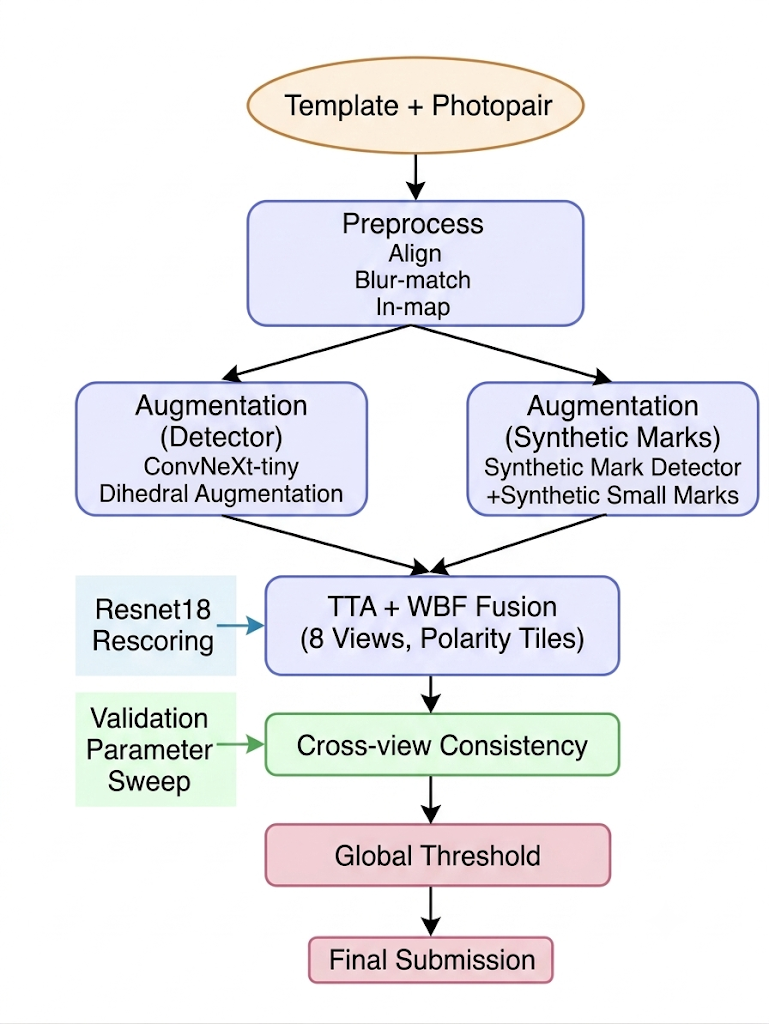
\includegraphics[width=0.38\textwidth]{task1_architecture.png}
\caption{Task~1 pipeline: preprocessing, a ten-detector Siamese CenterNet ensemble,
8-view TTA fused by WBF, five cross-fold ResNet-18 verifiers and the final decode
(threshold 0.43, swept on out-of-fold predictions).}
\label{fig:t1-arch}
\end{figure}

The pipeline (Fig.~\ref{fig:t1-arch}) has five stages.


\noindent\textbf{Stage 0: preprocessing.} A phase-correlation alignment check, with translation
correction if needed; blur matching of the template to the photo by a $\sigma$-grid
search on Laplacian variance; and a shadow- and tone-invariant \emph{ink map},
$\mathrm{GaussianBlur}(\mathrm{gray},\sigma{=}31) - \mathrm{gray}$.

\noindent\textbf{Stage 1: detector.} A Siamese ConvNeXt-Tiny~\cite{liu2022convnext} encoder with
shared weights over 4-channel (BGR~+~ink) streams, fused at every scale by
$\mathrm{conv}(\mathrm{concat}(a,b,|a-b|))$ and decoded through a
U-Net~\cite{ronneberger2015unet} path to \textbf{output stride 2} rather than the usual
4, to resolve the $8\times8$\,px boxes (stride~4 was not ablated). Four
CenterNet-style~\cite{zhou2019centernet} heads predict a centre heatmap, width/height,
a sub-pixel offset and an auxiliary change mask. Two training recipes $\times$ five
folds give ten detectors: \texttt{\_aug} uses the real training pairs with dihedral
augmentation, and \texttt{\_augsyn} adds fold-scoped synthetic small-mark pairs
(Exp.~A5).

\noindent\textbf{Stage 2: TTA fusion.} Each detector runs on 8 dihedral views, fused with Weighted
Boxes Fusion~\cite{solovyev2021wbf}; the detectors' fused outputs are then pooled.

\noindent\textbf{Stage 3: verifier.} A ResNet-18~\cite{he2016resnet} on $96\times96$ crops with an
8-channel stem produces a real-difference probability, blended with the detector
score, and a box-delta refinement. Five verifiers are trained strictly cross-fold.

\noindent\textbf{Stage 4: final decode.} A polarity filter (no pure-deletion class exists in the
data), ink-map snapping with a measured margin, and one global score threshold (0.43),
swept only on out-of-fold predictions.
% TODO: confirm in the code that polarity filter and snapping run after the verifier, as written here

\noindent\textbf{Submission.} The submission contains 668 boxes over the 100 test
images (6.68 per image, against a training average of 7.04), from all ten detectors
with TTA and all five verifiers averaged. The out-of-fold evaluation used a smaller
system (per fold, one detector of each recipe and one verifier), so the official score
is the only estimate that covers the submitted system.

\noindent\textbf{Leakage discipline.} (1)~Synthetic pairs are fold-scoped: each fold
discards the synthetic pairs derived from its own validation pages (836--892 of
6{,}400 per fold). (2)~Unlabelled test templates, which carry no labels, are used as a
synthesis source; no test photographs are used for threshold selection. (3)~The verifier for fold~$k$ trains only on candidates from folds
$\neq k$, produced by detectors that never saw those pages. (4)~The global threshold is
swept on out-of-fold predictions only, never on the reported fold or the test set.
% TODO: confirm that only templates, not test photographs, entered synthesis

\subsection{Development Path}
\label{sec:t1-experiments}

From the first Siamese CenterNet (fold-0 F1 0.9049) to the pooled detector-plus-verifier
system (0.9465), four observations decided the design; Table~\ref{tab:t1-path} in
Appendix~\ref{app:t1} traces every step.


\noindent\textbf{Precision is the hard part.} A classical difference baseline reaches
recall 0.572 but F1 0.0293, because every glyph edge fires in the blurrier photo
(Exp.~A1). Blur matching and the ink map of Stage~0 follow from this.

\noindent\textbf{Model and decode are entangled.} The same \texttt{\_aug} weights
scored 0.9049 at the original decode and 0.9257 with a lower threshold, a larger box
cap and 8-view TTA (Exp.~A6), so earlier ``no gain'' verdicts had compared decoders as
much as models.

\noindent\textbf{The recall ceiling, not F1, chose the ensemble.} The fraction of
ground-truth boxes present anywhere in the candidate list bounds every rescoring
idea. \texttt{\_augsyn} has worse standalone F1 (0.896 against 0.926) but raises the
ceiling from 0.9440 to 0.9590, and on boxes under 12\,px from 0.891 to 0.922
(Exps.~A5, A8). The two-family ensemble adds only 0.001 F1 but lifts the ceiling to
0.963, leaving the verifier to do the rescoring (Exp.~A9). The verifier first gave
$+0.0009$ because it was trained on filtered, capped candidates with almost no real
negatives (Exp.~A10); retrained on about 11{,}000 raw candidates per fold at 8:1
negatives to positives, it improved every fold, by $+0.006$ to $+0.018$ (Exp.~A11).

\noindent\textbf{Silent bugs made working ideas look like failures} (Exps.~A16--A18).
Fused WBF confidence was computed as
$\mathrm{sum(scores)}/\min(\mathrm{members}{+}1,3)$, which clipped well-supported boxes
to 1.0 while single-view boxes kept their raw score, so 8-view TTA scored F1 0.775,
worse than no TTA. The ensemble also double-counted its sources, collapsing recall to
0.056, and a verifier loader that re-decoded full pages took about 60 minutes per epoch
with the GPU idle. All numbers from Exp.~A6 onwards were produced after the fixes;
the size-relative box loss (A3) and EMA weights (A4) predate them, showed no effect and
were not repeated.

\subsection{Results}
\label{sec:t1-results}

The organisers scored the submission at accuracy 0.9577, precision 0.9656, recall
0.9499 and F$_\beta$ 0.9577 (Table~\ref{tab:t1-results}); they released only these
rounded metrics, not confusion counts. With 668 predictions, back-solving from the
rounded precision and recall gives TP~$\approx$645, FP~$\approx$23 and FN~$\approx$34
(implying about 679 ground-truth boxes and $F_1=1290/1347$). These are approximate
reconstructions, accurate only up to the rounding of the official figures, not
reported counts. That is roughly 57 errors, where F1~$=$~0.97 would have needed about
40 total errors (at most 39 to exceed 0.97, since $2\cdot654/1347=0.9711$). The larger
submitted ensemble is consistent with
the upside we wrote down before the results were released, but we cannot separate it
from test-set difficulty. Per-fold F1 was 0.943, 0.955, 0.935, 0.961 and 0.968. Threshold-selection optimism, measured by
nested cross-validation, is 0.0030 (Exp.~A13). Checkpoint selection inflates the
undertrained \texttt{\_augsyn} models by $+0.034$ on average (Exp.~A14), but the
official score still exceeded the raw out-of-fold F1.

\begin{table}[t]
\caption{Task 1 results. $^\dagger$Approximate reconstruction from the official precision, recall and the 668 predictions; the organisers did not release confusion counts.}\label{tab:t1-results}
\centering
\small\setlength{\tabcolsep}{4pt}
\begin{tabular}{lcccccc}
\toprule
Configuration & F1 & Prec. & Rec. & TP & FP & FN \\
\midrule
\textbf{Official test (accuracy $=$ F1)} & \textbf{0.9577} & 0.9656 & 0.9499 & $\approx$645$^\dagger$ & $\approx$23$^\dagger$ & $\approx$34$^\dagger$ \\
Nested out-of-fold (threshold-bias-corrected) & 0.9435 & --- & --- & --- & --- & --- \\
Pooled out-of-fold, detector + verifier (A12) & 0.9465 & 0.963 & 0.930 & 1{,}309 & 50 & 98 \\
Pooled out-of-fold, detector only (A13) & 0.9385 & --- & --- & --- & --- & --- \\
Fold-0 starting point (A2) & 0.9049 & 0.922 & 0.888 & 238 & 20 & 30 \\
Perfect-rescorer ceiling (A15) & 0.9801 & 1.000 & 0.961 & 1{,}352 & 0 & 55 \\
\midrule
\multicolumn{7}{l}{Competition target: 0.97 (not reached; practically out of reach with these proposals)} \\
\bottomrule
\end{tabular}
\end{table}

\noindent\textbf{Qualitative results.} Fig.~\ref{fig:t1-qual} shows example
out-of-fold predictions: correct detections, false positives, boxes that no model
proposes (the 55 boxes of Exp.~A15), and candidates whose score the verifier changed
(Exp.~A11).
% TODO: replace the four placeholder images (task1_qual_*.png) with real crops and
% describe what each panel shows (box size, polarity, why it is missed or rejected).

\begin{figure}[t]
\centering
\begin{minipage}[t]{0.48\textwidth}\centering
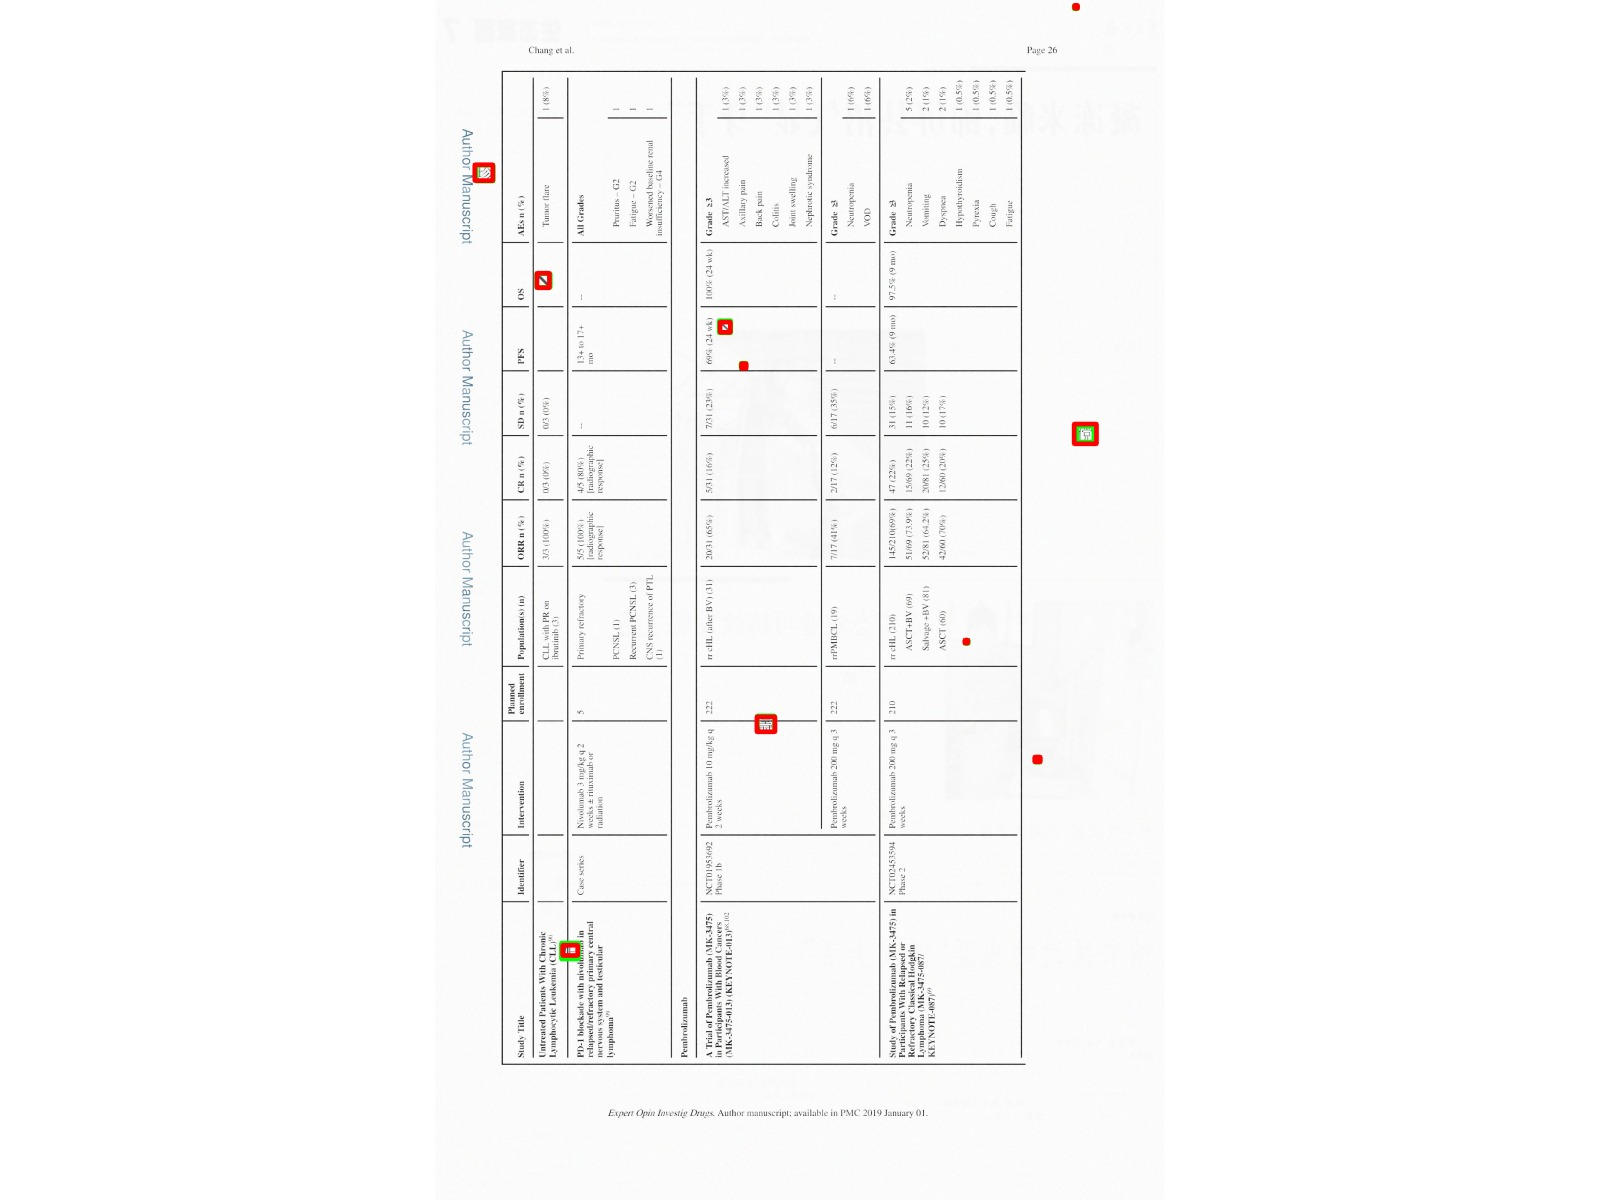
\includegraphics[width=\linewidth]{task1_qual_tp.png}\\[-1pt]
{\small (a) Correct detections}
\end{minipage}\hfill
\begin{minipage}[t]{0.48\textwidth}\centering
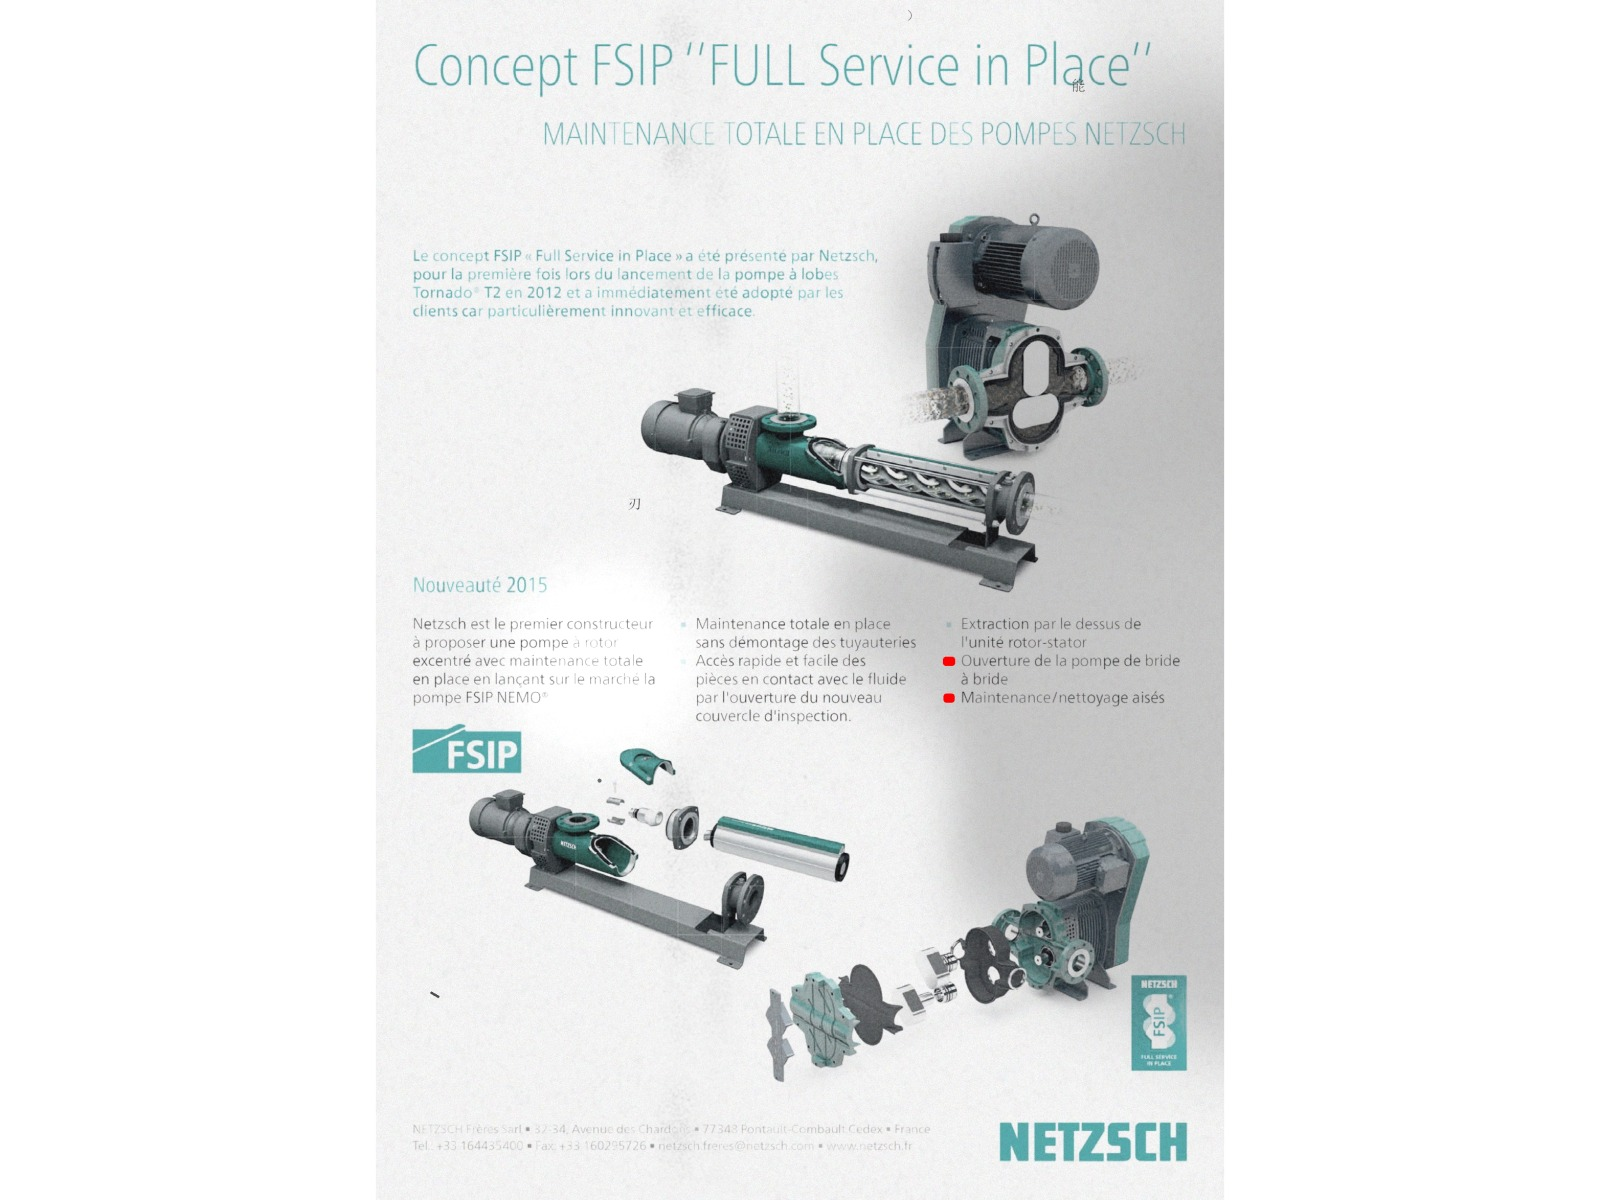
\includegraphics[width=\linewidth]{task1_qual_fp.png}\\[-1pt]
{\small (b) False positives}
\end{minipage}\\[6pt]
\begin{minipage}[t]{0.48\textwidth}\centering
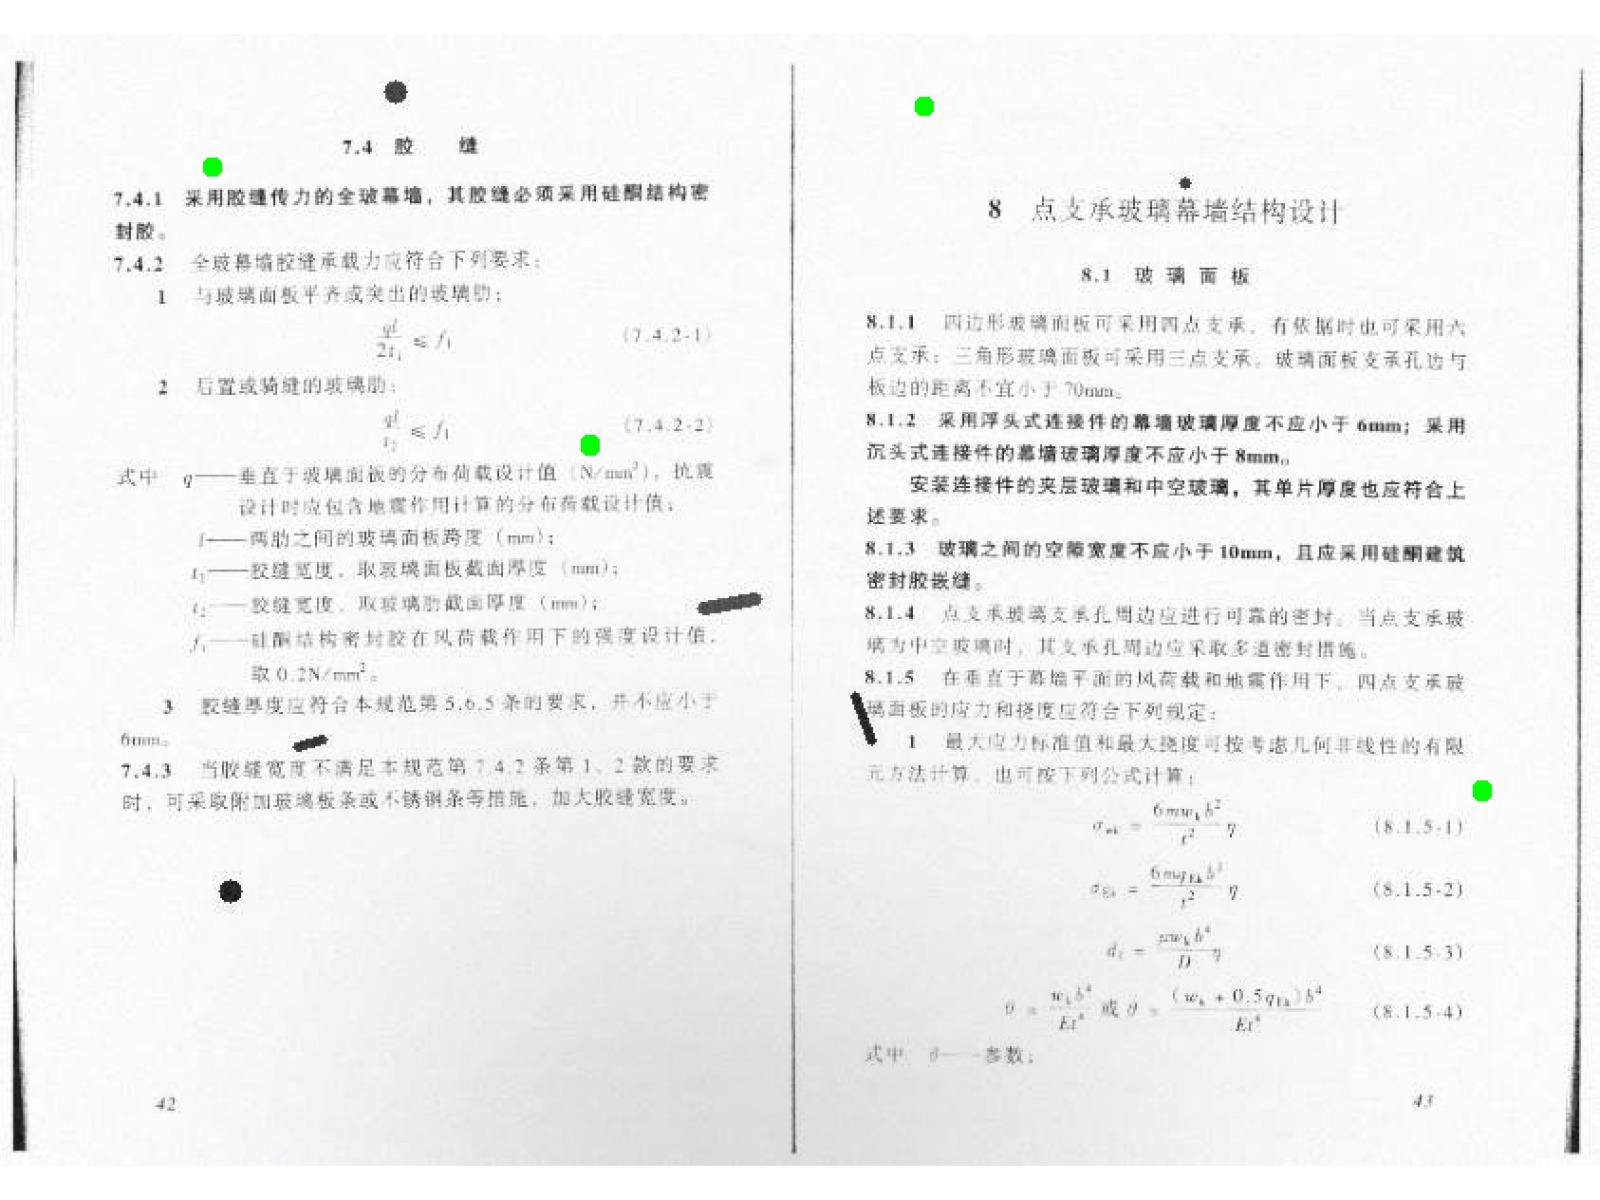
\includegraphics[width=\linewidth]{task1_qual_missed.png}\\[-1pt]
{\small (c) Missed boxes (never proposed)}
\end{minipage}\hfill
\begin{minipage}[t]{0.48\textwidth}\centering
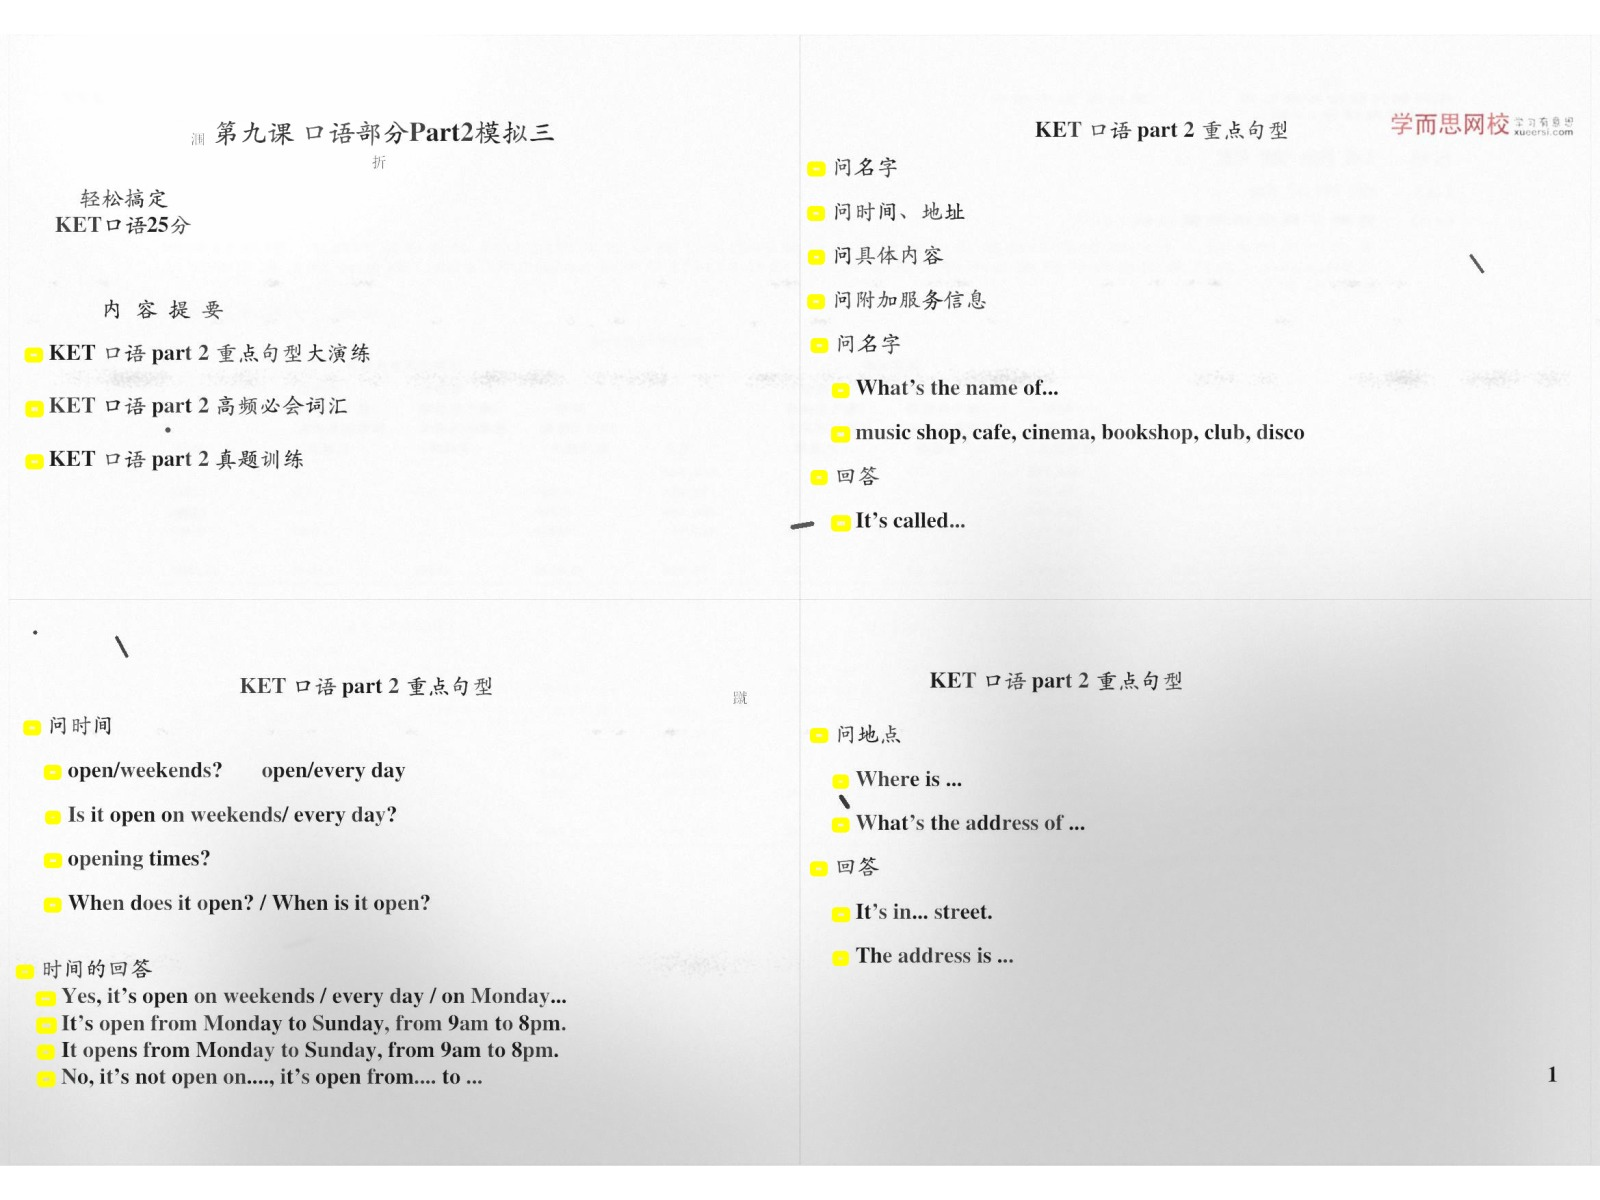
\includegraphics[width=\linewidth]{task1_qual_verifier.png}\\[-1pt]
{\small (d) Verifier corrections}
\end{minipage}
\caption{Task~1 qualitative results on out-of-fold predictions, with ground-truth and
predicted boxes overlaid on each pair.}
\label{fig:t1-qual}
\end{figure}

\noindent\textbf{Reachability of 0.97.} The final candidate set contains 1{,}352 of
the 1{,}407 boxes, so even a perfect rescorer caps at F1 0.9801 (Exp.~A15). The target
lies below this ceiling, but keeping all 1{,}352 matching proposals would still allow
at most about 28 false positives, against 50 out of fold, and the achieved 0.9465 is
0.0336 below the ceiling. Further gains need better proposals for the 55 boxes no
model finds, not better verifiers.

\noindent\textbf{Limitations.} Stride~2, the ink map, Siamese fusion, the polarity
filter, ink-map snapping and box-delta refinement were design choices that were not
ablated individually. Fold-0 comparisons rest on 268 boxes with no multi-seed noise
estimate. Exps.~A3 and~A4 were not repeated under the corrected fusion.
